\documentclass[iop,numberedappendix,apj,onecolumn]{emulateapj}
%\documentclass[iop,numberedappendix,apj]{aastex}
%\documentclass{article}
%\usepackage{emulateapj}
%\pdfoutput=1
\usepackage{color}
\usepackage{amssymb}
%\PassOptionsToPackage{hyphens}{url}
\usepackage{hyperref}
%\usepackage{breakurl}
\def\UrlBreaks{\do\/\do-}
\usepackage{natbib}
\usepackage{graphicx}
\usepackage{epsfig}
%\usepackage[hyphens]{url}
%\usepackage{csquotes}
%\usepackage{lscape}
\usepackage{afterpage}

\usepackage[tbtags]{amsmath}
\usepackage{hyperref,xcolor}
\hypersetup{colorlinks,linkcolor={blue!50!black},citecolor={blue!50!black},urlcolor={blue!80!black}}
\setlength{\tabcolsep}{0.04in} 
%\usepackage{epsfig}
%\usepackage{fullpage}
%\usepackage{hyperref}
%%%%%%%%%%%%%%%%%%%%%%%%%%%%%%%%%%%%%%%%%%%%%%%%%%%%%%%%%%%%%%%%%%%%%%%%%%%%%%%
%%% NOTES ON COMPILING / PRINTING THIS DOCUMENT
%%% do the latex <filename>
%%% dvips -O 0cm,2.0cm <filename.dvi>
%%% dvips -O 0cm,2.0cm clash_pressures.dvi

\newcommand {\apgt} {\ {\raise-.5ex\hbox{$\buildrel>\over\sim$}}\ }
\newcommand {\aplt} {\ {\raise-.5ex\hbox{$\buildrel<\over\sim$}}\ }
\newcommand{\dmod}{\overrightarrow{d}_{mod}}
\newcommand{\dvec}{\overrightarrow{d}}
\newcommand{\avec}{\overrightarrow{a}}
\newcommand{\asec}{$^{\prime \prime}$}
\newcommand{\asecs}{$^{\prime \prime}\ $}
\newcommand{\amin}{$^{\prime}$}
\newcommand{\amins}{$^{\prime}\ $}
\newcommand{\sigT}{\mbox{$\sigma_{\mbox{\tiny T}}$}}
\newcommand{\Tcmb}{\mbox{$T_{\mbox{\tiny CMB}}$}}
\newcommand{\kB}{\mbox{$k_{\mbox{\tiny B}}$}}
\newcommand{\kBT}{\mbox{$k_{\mbox{\tiny B}}T_{\mbox{\tiny e}}$}}
\newcommand{\nH}{\mbox{$n_{\mbox{\tiny H}}$}}
\newcommand{\NH}{\mbox{$N_{\mbox{\tiny H}}$}}
\newcommand{\LameH}{\mbox{$\Lambda_{e \mbox{\tiny H}}$}}
\newcommand{\Lamee}{\mbox{$\Lambda_{ee}$}}
\newcommand{\rhogas}{\mbox{$\rho_{\mbox{\scriptsize gas}}$}}
\newcommand{\rhotot}{\mbox{$\rho_{\mbox{\scriptsize tot}}$}}
\newcommand{\Mgas}{\mbox{$M_{\mbox{\scriptsize gas}}$}}
\newcommand{\Mtot}{\mbox{$M_{\mbox{\scriptsize tot}}$}}
\newcommand{\Mvir}{\mbox{$M_{\mbox{\scriptsize vir}}$}}
\newcommand{\Yint}{\mbox{$Y_{\mbox{\scriptsize int}}$}}
\newcommand{\Ycyl}{\mbox{$Y_{\mbox{\scriptsize cyl}}$}}
\newcommand{\Ysph}{\mbox{$Y_{\mbox{\scriptsize sph}}$}}
\newcommand{\fgas}{\mbox{$f_{\mbox{\scriptsize gas}}$}}
\newcommand{\LCDM}{\mbox{$\Lambda$CDM}}
\newcommand{\Pe}{\mbox{$P_{\mbox{\scriptsize e}}$}}
\newcommand{\msun}{$M_{\odot}$}
\newcommand{\etal}{{\it et al.}}
\newcommand{\mJy}{\,{\rm mJy} }
\newcommand{\um}{\,\mu {\rm m} }
\newcommand{\mJySr}{\,{\rm MJy/Sr} }
\newcommand{\mJyBm}{\,{\rm mJy/Bm} }
\newcommand{\mK}{\,{\rm mK} }
\newcommand{\K}{\,{\rm K} }
\newcommand{\uJy}{\,{\rm \mu Jy} }
\newcommand{\uK}{\,{\rm \mu K} }
\newcommand{\kHz}{\, {\rm kHz} }
\newcommand{\eg}{{\it e.g.}}
\newcommand{\ie}{{\it i.e.}}
\newcommand{\etc}{{\it etc.}}
\newcommand{\aips}{{\tt AIPS++}}
\newcommand{\nusp}{\nu_{sp}}
\newcommand{\ghz}{{\, \rm GHz}}
\newcommand{\db}{{\, \rm dB}}
\newcommand{\degsqr}{\, {\rm deg^2}}
\newcommand{\Tew}{\mbox{$T_{\mathrm{ew}}$}}
\newcommand{\Tspec}{\mbox{$T_{\mathrm{spec}}$}}
\newcommand{\chandra}{{\it Chandra}}
\newcommand{\asca}{{ASCA}}
\newcommand{\wmap}{{WMAP}}
\newcommand{\rosat}{{ROSAT}}
\newcommand{\xmm}{{XMM-{\it Newton}}}
\newcommand{\planck}{{\it Planck}}
\newcommand{\hubble}{{\it Hubble}}
\newcommand{\rxj}{RX J1347.5-1145}
\newcommand{\clj}{CL J1226.9+3332}
\newcommand{\macsa}{MACS J0647.7+7015}
\newcommand{\macsb}{MACS J1206.2-0847}
\newcommand{\macsc}{MACS J0717.5+3745}
\newcommand{\macsd}{MACS J1423.8+2404}
\newcommand{\macse}{MACS J0329.6-0211}
\newcommand{\macsf}{MACS J0429-0253}
\newcommand{\macsg}{MACS J0744.9+3927}
\newcommand{\macsh}{MACS J1149+2223}
\newcommand{\macsi}{MACS J1115+0130}
\newcommand{\Tx}{\mbox{$T_{\mbox{\tiny X}}$}}
\newcommand{\te}{\mbox{$T_{\mbox{\tiny e}}$}}
\newcommand{\mec}{\mbox{$m_{\mbox{\tiny e}} c^2$}}
\newcommand{\dene}{\mbox{$n_{\mbox{\tiny e}}$}}
\newcommand{\denesq}{\mbox{$n^2_{\mbox{\tiny e}}$}}
\newcommand{\yx}{\mbox{$Y_{\mbox{\tiny X}}$}}
\newcommand{\ysze}{\mbox{$Y_{\mbox{\tiny tSZE}}$}}
\newcommand{\sx}{\mbox{$S_{\mbox{\tiny X}}$}}
\newcommand{\Itsz}{\mbox{$I_{\mbox{\tiny tSZE}}$}}
\newcommand{\Iksz}{\mbox{$I_{\mbox{\tiny kSZE}}$}}
\newcommand{\chisq}{\mbox{$\chi^{2}$}}
\newcommand{\chired}{\mbox{$\chi^{2}_{red}$}}

\defcitealias{arnaud2010}{A10}
\defcitealias{cavagnolo2009}{C09}
\defcitealias{bulbul2010}{B10}
\defcitealias{vikhlinin2006}{V06}

\newcommand{\quotes}[1]{``#1''}

\slugcomment{}
\shortauthors{Romero \etal}
\shorttitle{Memo: Maximum Likelihood Deprojection}
%altaffilmark{#}

\begin{document}

\title{Maximum Likelihood Deprojection of CLJ1226.9 with NIKA}
\author{
%  Order TBD ,
  Charles E. Romero\altaffilmark{1,2,3},
  Matthew McWilliam \altaffilmark{4},
  Juan Macias-Perez \altaffilmark{4},
  NIKA Collaboration \altaffilmark{4}
} 
\date{\today}

%%%%%%%%%%%%%%%%%%%%%%%%%%%%%%%%%%%%%%%%%%%%%%%%%%%%%%%%%%%%%%%%%%%%%%%%%%%%%%%
\altaffiltext{1}{Institut de Radioastronomie Millim\'{e}trique
300 rue de la Piscine, Domaine Universitaire
38406 Saint Martin d'H\`{e}res, France} 
\altaffiltext{2}{Department of Astronomy, University of Virginia,
  P.O. Box 400325, Charlottesville, VA 22904, USA}
\altaffiltext{3}{National Radio Astronomy Observatory, 520 Edgemont Rd.,
Charlottesville, VA 22904, USA}
\altaffiltext{4}{Department of Physics, Math, and Astronomy,
  California Institute of Technology, Pasadena, CA 91125, USA}
\altaffiltext{5}{Author contact: \email{romero@iram.fr}}
%\begin{document}

%%%%%%%%%%%%%%%%%%%%%%%%%%%%%%%%%%%%%%%%%%%%%%%%%%%%%%%%%%%%%%%%%%%%%%%%%%%%%%%

\begin{abstract}
We explore the ability to deproject SZ maps into non parametric pressure profiles. 
\end{abstract}

\keywords{galaxy clusters: individual: CLJ1226.9+3352}

\maketitle

%%%%%%%%%%%%%%%%%%%%%%%%%%%%%%%%%%%%%%%%%%%%%%%%%%%%%%%%%%%%%%%%%%%%%%%%%%%%%%%
\section{Introduction}
\label{sec:intro}
%%%%%%%%%%%%%%%%%%%%%%%%%%%%%%%%%%%%%%%%%%%%%%%%%%%%%%%%%%%%%%%%%%%%%%%%%%%%%%%

%%%%%%%%%%%%%%%%%%%%%%%%%%%%%%%%%%%%%%%%%%%%%%%%%%%%%%%%%%%%%%%%%%%%%%%%%%%%%%%
\section{Maximum Likelihood Deprojection Technique with NIKA}
\label{sec:ml_dep_NIKA}
%%%%%%%%%%%%%%%%%%%%%%%%%%%%%%%%%%%%%%%%%%%%%%%%%%%%%%%%%%%%%%%%%%%%%%%%%%%%%%%

\subsection{Overview}
\label{sec:jf_overview}

Deproction by maximum likelihood is simply a fitting routine which models a cluster
with $N$ individual pressure bins. That is, the pressure bins (spherical shells)
are integrated along the line of sight, converted to a Compton y map, on the sky.
This map is then convolved with the instrument's beam and transfer function.

We start with NIKA data, as it has the strongest map significance (and overall
detection significance) to get a sense of how our technique performs. In
Figure~\ref{fig:virtual_fits}, we have fit our (projected) pressure shells to
a virtual map (a model from a previous study, plus noise).

\begin{figure}[!h]
  \centering
  \begin{tabular}{cc}
   \epsfig{file=NIKA_ml_deproj_figs/NIKA_VB_6_B_2500S_250B_30W_pressure.eps,width=0.50\linewidth,clip=} &
   \epsfig{file=NIKA_ml_deproj_figs/NIKA_VB_6_B_2500S_250B_30W_contour.eps,width=0.50\linewidth,clip=} 
  \end{tabular}
  \caption{Our maximum likelihood fits to NIKA virtual data. We used 6 bins, 2500 steps, 250 of which were
    burn in. 30 walkers were used. No mean level was fit.
    The error bars on the second bin appears much large than it should be.
    However, it could also be that the error bar on the first bin is artificially small.}
  \label{fig:virtual_fits}
\end{figure}

\newpage

Two problems which we are currently trying to resolve are:
\begin{enumerate}
  \setlength{\itemsep}{0pt}
  \setlength{\parskip}{0pt}
  \item Error bars don't appear accurate to be accurate. \\
  \item Profile fits at large radii in NIKA (and Bolocam) had, at some point, been too large.
\end{enumerate}

Some potential issues to be (double) checked:
\begin{enumerate}
  \setlength{\itemsep}{0pt}
  \setlength{\parskip}{0pt}
  \item Is the point source being subtracted \\
  \begin{itemize}
    \item \textcolor{red}{Yes, as a simple Gaussian.}
  \end{itemize}
  \item Do we need to account for a mean level?
  \begin{itemize}
    \item \textcolor{red}{Maybe, but I think the below analysis says this is not the ``right'' way to do it.}
  \end{itemize}
 
\end{enumerate}

What's left to be considered are:

\begin{enumerate}
  \setlength{\itemsep}{0pt}
  \setlength{\parskip}{0pt}
  \item Using Planck constraints
  \begin{itemize}
    \item \textcolor{red}{I think this is the best approach.}
  \end{itemize}
  \item Restricting the outer profile but some other prior (going to ``zero'' at some radius).
  \begin{itemize}
    \item \textcolor{red}{I don't like it, and I don't think it'd work, but it is a last resort.}
  \end{itemize}
\end{enumerate}

\newpage

\subsection{Mean Level}
\label{sec:mean_level}

%%% JSayers: Bolocam too? Yes...if done, both are done. But I removed the mean level fit in the simple sense.
%%% I don´t think I fit out a Bolocam mean level, because it was so low.
Similar to \citet{czakon2015}, we wish to account for a mean level (signal offset) in the MUSTANG maps.
We do not wish to fit for a mean level simultaneously as a bulk component given the degeneracies. Therefore,
to determine the mean level independent of the other components, we create a MUSTANG noise map
% from time-flipped TOD 
and calculate the mean within the inner arcminute for each cluster. This mean is then subtracted before 
the other components are fit. 

\subsubsection{Point Sources}
\label{sec:ptsrcs}

For MUSTANG, point sources are treated in the same manner as in \citet{romero2015a}. 
A point source is identified by NIKA \citep{adam2015} in CLJ1226, which is posited to
be a submillimeter galaxy (SMG) behind the cluster. We fix the point source amplitude
in the NIKA map to that found in \citet{adam2015}. As of November 2016, the point source
subtraction and beam convolutions are performed with a simple (single) Gaussian. However,
we look to use a more accurate beam (probably a double Gaussian).

%%%%%%%%%%%%%%%%%%%%%%%%%%%%%%%%%%%%%%
For the Bolocam image

\subsubsection{Centroid}

The default centroids used when gridding our bulk ICM component are the ACCEPT centroids. Given the offsets
between ACCEPT and Bolocam centroids (Table~\ref{tbl:cluster_properties}), we perform a second set of
fits where we grid the bulk ICM component using the Bolocam centroids. The ACCEPT centroid are taken to be the
X-ray peaks unless their centroiding algorithm produced a centroid more than 70 kpc from the X-ray peak, in which
case they adopt that centroid \citep{cavagnolo2008a}. 
%We do not find significant changes in
%the fitted gNFW parameters (Section~\ref{sec:pp_constraints}), 

%%%%%%%%%%%%%%%%%%%%%%%%%%%%%%%%%%%%%%%%%%%%%%%%%%%%%%%%%%%%%%%%%%%%%%%%%%%%%%%%%%%%%%%%%%%%%%%%%%%%%%%%%%%
%%%                                                SOME FIGURES                                         %%%
%%%%%%%%%%%%%%%%%%%%%%%%%%%%%%%%%%%%%%%%%%%%%%%%%%%%%%%%%%%%%%%%%%%%%%%%%%%%%%%%%%%%%%%%%%%%%%%%%%%%%%%%%%%

\begin{figure}[!h]
  \centering
  \begin{tabular}{cc}
   \epsfig{file=NIKA_ml_deproj_figs/NIKA_RB_6_B_2000S_250B_30W_pressure.eps,width=0.50\linewidth,clip=} &
   \epsfig{file=NIKA_ml_deproj_figs/NIKA_RB_6_B_3000S_500B_30W_pressure.eps,width=0.50\linewidth,clip=} \\
   \epsfig{file=NIKA_ml_deproj_figs/NIKA_RB_6_B_2000S_250B_30W_contour.eps,width=0.50\linewidth,clip=} &
   \epsfig{file=NIKA_ml_deproj_figs/NIKA_RB_6_B_3000S_500B_30W_contour.eps,width=0.50\linewidth,clip=} 
  \end{tabular}
  \caption{Deprojected results when fitting to \textbf{real} NIKA data. Here we used 6 bins, 2000-3000 steps,
    250-500 of which were burn-in steps, and 30 walkers.
    The left panels show results to NIKA (real) data with no mean level subtraction. The right panels
    show the same results, but with a fitted mean level.}
  \label{fig:mn_lvl_comparison}
\end{figure}

%%%%%%%%%%%%%%%%%%%%%%%%%%%%%%%%%%%%%%%%%%%%%%%%%%%%%%%%%%%%%%%%%%%%%%%%%%%%%%%
\newpage
\subsection{Extra Confusion}
\label{sec:confusion}
%%%%%%%%%%%%%%%%%%%%%%%%%%%%%%%%%%%%%%%%%%%%%%%%%%%%%%%%%%%%%%%%%%%%%%%%%%%%%%%

Ah, but why do the fits change so much on the virtual data when I try to fit a mean level??? This should
suggest that the problem is with the fitting algorithm somehow. But...how? And why (as evidenced in
Section~\ref{sec:must_bolo}) is it such a problem for NIKA as compared to MUSTANG or Bolocam?

\begin{figure}[!h]
  \centering
  \begin{tabular}{cc}
   \epsfig{file=NIKA_ml_deproj_figs/NIKA_VB_6_B_2400S_400B_30W_pressure.eps,width=0.50\linewidth,clip=} &
   \epsfig{file=NIKA_ml_deproj_figs/NIKA_VB_6_B_2400S_400B_30W_contour.eps,width=0.50\linewidth,clip=} 
  \end{tabular}
  \caption{Deprojected results when fitting to virtual NIKA data. Here we used 6 bins, 2400 steps,
    400 of which were burn-in steps, and 30 walkers.
    This shows the same symptoms as the real data!!! That was unexpected! But then, this strongly
    points to an issue in the algorithm over an issue in the real data.}
  \label{fig:virtual_fits}
\end{figure}

%%%%%%%%%%%%%%%%%%%%%%%%%%%%%%%%%%%%%%%%%%%%%%%%%%%%%%%%%%%%%%%%%%%%%%%%%%%%%%%
\newpage
\subsection{Fits with MUSTANG and Bolocam}
\label{sec:must_bolo}
%%%%%%%%%%%%%%%%%%%%%%%%%%%%%%%%%%%%%%%%%%%%%%%%%%%%%%%%%%%%%%%%%%%%%%%%%%%%%%%

\subsubsection{MUSTANG}

In Figure~\ref{fig:mustang_fits}, it is clear that trying to fit for a mean level with MUSTANG data is not
appropriate, at least not without any other constraints. The (real) MUSTANG map already has the point source
subtracted and the mean level subtracted (see Romero+ 2016 for how the mean level is calculated.)

\begin{figure}[!h]
  \centering
  \begin{tabular}{cc}
   \epsfig{file=NIKA_ml_deproj_figs/MUSTANG_VB_6_B_2400S_400B_30W_pressure.eps,width=0.50\linewidth,clip=} &
   \epsfig{file=NIKA_ml_deproj_figs/MUSTANG_VB_6_B_2400S_400B_ML-NO_30W_pressure.eps,width=0.50\linewidth,clip=} 
  \end{tabular}
  \caption{Deprojected MUSTANG results when fit to virtual data. Here we used 6 bins, 2400 steps, 400 of which
    were burn in, and 30 walkers.
    The left hand panel shows the deprojected pressure profiles when a mean level is also fit. The right hand
    side shows the fits without fitting for a mean level.}
  \label{fig:mustang_fits}
\end{figure}

\subsubsection{Bolocam}

In Figure~\ref{fig:bolocam_fits}, we find that fittin for a gmean level with Bolocam data does not appear
to be problematic. However, the (real) Bolocam map already has the mean level subtracted
\citep{czakon2015}.

\begin{figure}[!h]
  \centering
  \begin{tabular}{cc}
   \epsfig{file=NIKA_ml_deproj_figs/BOLOCAM_VB_6_B_2400S_400B_30W_pressure.eps,width=0.50\linewidth,clip=} &
%   \epsfig{file=NIKA_ml_deproj_figs/MUSTANG_VB_6_B_2400S_400B_ML-NO_30W_pressure.eps,width=0.50\linewidth,clip=} 
  \end{tabular}
  \caption{Deprojected Bolocam results when fit to virtual data. Here we used 6 bins, 2400 steps, 400 of which
    were burn in, and 30 walkers.
    The left hand panel shows the deprojected pressure profiles when a mean level is also fit. The right hand
    side shows the fits without fitting for a mean level.}
  \label{fig:bolocam_fits}
\end{figure}


%%%%%%%%%%%%%%%%%%%%%%%%%%%%%%%%%%%%%%%%%%%%%%%%%%%%%%%%%%%%%%%%%%%%%%%%%%%%%%%
\section{Augmented Outputs}
\label{sec:augmentation}
%%%%%%%%%%%%%%%%%%%%%%%%%%%%%%%%%%%%%%%%%%%%%%%%%%%%%%%%%%%%%%%%%%%%%%%%%%%%%%%

%%%%%%%%%%%%%%%%%%%%%%%%%%%%%%%%%%%%%%%%%%%%%%%%%%%%%%%%%%%%%%%%%%%%%%%%%%%%%%%
\section{Covariance}
\label{sec:covariance}
%%%%%%%%%%%%%%%%%%%%%%%%%%%%%%%%%%%%%%%%%%%%%%%%%%%%%%%%%%%%%%%%%%%%%%%%%%%%%%%

\begin{table}
  \centering
  \begin{tabular}{c c c c}
    1.    & -0.68 &  0.35 &  0.33 \\
    -0.68 &  1.   & -0.53 & -0.48 \\
    0.35  & -0.53 &  1.   &  0.94 \\
    0.33  & -0.48 &  0.94 &  1.
  \end{tabular}
  \caption{Correlation matrix for Bolocam (4 bins, clearly).}
\end{table}
%[ 1.  , -0.8 ,  0.43, -0.16],
%       [-0.8 ,  1.  , -0.74,  0.36],
%       [ 0.43, -0.74,  1.  , -0.58],
%       [-0.16,  0.36, -0.58,  1.  ]])
%%%%%%%%%%%%%%%%%%%%%%%%%%%%%%%%%%%%%%%%%%%%%%%%%%%%%%%%%%%%%%%%%%%%%%%%%%%%%%%%%%%%%%%%%%%%%%%%%%%%%%%%%%%%%%%%
%%%%%%%%%%%%%%%%%%%%%%%%                    CONCLUSIONS!!!                           %%%%%%%%%%%%%%%%%%%%%%%%%%%
%%%%%%%%%%%%%%%%%%%%%%%%%%%%%%%%%%%%%%%%%%%%%%%%%%%%%%%%%%%%%%%%%%%%%%%%%%%%%%%%%%%%%%%%%%%%%%%%%%%%%%%%%%%%%%%%

\section{Conclusions}
\label{sec:conclusions}

We developed an algorithm. It requires a lot of testing. It behaves unexepectedly.

%%%%%%%%%%%%%%%%%%%%%%%%%%%%%%%%%%%%%%%%%%%%%%%%%%%%%%%%%%%%%%%%%%%%%%%%%%%%%%%%%%%%%%%%%%%%%%%%%%%%%%%%%%%%%%%%
%%%%%%%%%%%%%%%%%%%%%%%%                    BIBLIOGRAPHY!!!                          %%%%%%%%%%%%%%%%%%%%%%%%%%%
%%%%%%%%%%%%%%%%%%%%%%%%%%%%%%%%%%%%%%%%%%%%%%%%%%%%%%%%%%%%%%%%%%%%%%%%%%%%%%%%%%%%%%%%%%%%%%%%%%%%%%%%%%%%%%%%


\bibliographystyle{apj}
\bibliography{mycluster}
\label{references}

\end{document}


